% ============================================================
% 4.1 FIELD EFFECTS (first part) -- Writer: Ignacio Gimeno -- about 290 words
% Template: present each result together with its interpretation, evidence and
% significance; refer to every figure in the text and say what the reader
% should see in it; distinguish observation from conclusion.
% Numbers: results/progress_stats.json (decomposition), results/final_figures_stats.json
% (fig1), results/final_fig1_field_effects.csv, figures/final/CAPTIONS.md.
% Start from outline entries 6 and 6a.
% ============================================================

\guide{Ignacio -- Opening of Section 4 (two sentences)}{%
Tell the reader the order of the section: what is measured (\S\ref{sec:res-field}), whether it persists and predicts (\S\ref{sec:res-prediction}), whether intake explains it (\S\ref{sec:res-confounders}), what it does to selection and how to correct it (\S\ref{sec:res-selection}--\S\ref{sec:res-rules}), whether it appears in the US (\S\ref{sec:res-us}).}
\budget{50}{Ignacio}

\subsection{Field Explains Most Grade Differences Within Universities}
\label{sec:res-field}

\guide{Ignacio -- Paragraph: the decomposition}{%
\textbf{Claim (outline 6):} field explains most grade differences within each university, and each university adds its own stable pattern.\\
\textbf{Numbers:} university-year averages explain 20\% of all variation; of what is left, 65\% is a field effect shared by all universities, 28\% is specific to each university and 7\% is year-to-year noise; the university-specific part is significant ($F = 26.2$, $p < 0.001$, 1,409 df); 1,528 university-field cells.\\
\textbf{Interpretation:} the shared part is what a single national correction could remove; the 28\% needs university-specific information (link to \S\ref{sec:res-prediction}).}
\budget{110}{Ignacio}

\guide{Ignacio -- Paragraph: Figure~\ref{fig:field-effects}}{%
\textbf{What the reader should see:} a range of about one grade point between the most and least generous fields: Nursing $+0.53$ and Early childhood teaching $+0.46$ at the top; Architecture $-0.53$, Agriculture $-0.45$ and Economics $-0.39$ at the bottom; intervals are narrow (median half-width 0.05 points) so the order is not noise.\\
\textbf{Put the size in context:} the gap between the extremes is 1.06 points, about 1.7 times the typical spread of grades inside one field (median within-field standard deviation 0.62 points, from the quartiles of 11,738 records; \texttt{final\_figures\_stats.json}, fig1). So a student in a low-graded field needs a much higher position in their own degree to reach the same pooled rank.\\
\textbf{Avoid:} calling fields ``harder'' or ``easier'' (outline 2a).}
\budget{130}{Ignacio}

\begin{figure}[t]
  \centering
  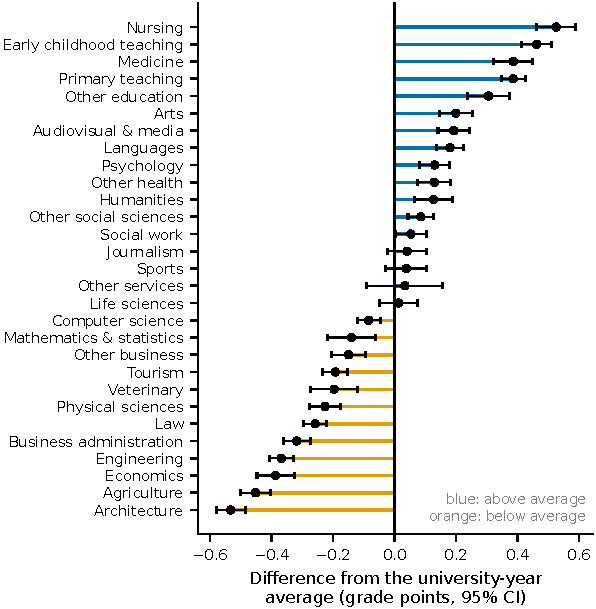
\includegraphics[width=\linewidth]{fig1_field_effects}
  \caption{\capguide{Ignacio -- see CAPTIONS.md, entry "Figure 1" (file fig1): what is shown (each field's distance from the average of all fields in the same university and year), data (SIIU, 12,125 means, 89 universities, 2015--16 to 2023--24, 5--10 scale), 95\% intervals clustered by university, colour meaning, source of the data.}}
  \label{fig:field-effects}
\end{figure}
